\chapter{Analysis}

\section{Introduction}

\subsection{Client Identification}

\begin{flushleft}

My client is Tom Henderson; he is thirty seven years old and is the principle veterinary surgeon and managing director of Beacon Veterinary. Tom graduated from Melbourne University, Victoria, Australia in 2000 and found employment with the Beacon Vet Centre in Aspatria in 2003. Since then Tom has brought partnership in the practice. \par 

As well as being the  principle surgeon, Tom also takes resposability for other roles, such as managing the businesses finance, organising staff payrolls and Managing the stock of the products they sell and equipment they use. On busy days, usually during the weekdays, Tom spends most of his working hours in the operating thetre. However, on less busy days or outside of opening hours, Tom spends time managing and organising the stock of the products the Veternary sell. To aid him, Tom uses an Edexcel Spreadsheet to record and track the stock of each product. \par 

Tom would like me to develop a new system for him because due to recent sucess in the business, Beacon Vets has introduced an increased range of  products available to sell. Tom has requested for this new system because he stated that his current system is now becoming too complicated and difficult to use now that the new products have been added. My client wants the new system to be easier to use and wants managing the stock to be a faster prcoess, so he doesn't have to spend as much time at the veternary centre and can spend more time with his children during the weekends.\par
\end{flushleft}

\subsection{Define the current system}

\begin{flushleft}
Despite being a veterinary centre, Beacon vets sold roughly a dozen products, such as Vetericyn, a non toxic cut / wound treatment for animals. The products sold at the Vets are usually products to maintain the animals health after an operation, however Beacon Vets are now selling products such as dietry foods and other products that customers can just come in and buy without coming  in to see the Vet. Because only a dozen items were being sold, and each customer never purchased over about 3 products, keeping track of the stock of each item used to be a relativly easy process. \par

Last year Beacon Vets expanded on the range of the products they sold, providing a wide variety of foods and treatments for all sorts of animals such as dogs, cats and rabbits etc. Although Beacon Vets greatly expanded on the products they sold, they did not change their system of keeping track of stock. The current system is a Microsoft Excel spreadsheet containing the information of the product, the selling price, the current amount in the front of the store, the current amount being stored in storage. This current system was useful and easy to use when handling a dozen products but has become difficult and confusing now many more products are being sold. here is the current Edexel Spreadsheet in use:\par
\end{flushleft}


\begin{figure}[H]

\hfill\includegraphics[width=14cm]{OldSystemExample.pdf}\hspace*{\fill}
\caption{An example of the current system being used.} \label{fig:Example Of Old System}
\end{figure}

\begin{flushleft}
Looking at \textit{Figure 1.1}, The current system is a basic spreadsheet created using Microsft Excel containing 4 columns and a row for each product. The column \textbf{\textit{item}}, contains the information to uniquely identify each product. Some of the data entered into the item comlumn can be be long because if the Veternary sells different quantities or weights of the ptoduct, then this is specified in this column. the column \textbf{\textit{price}}, is used make sure that the item being edited is correct. This coumn is usually only used when a specif product has either two quantites or weights and the \textbf{\textit{price}} column is used to second check that the right product is being edited. The \textbf{\textit{front stock}} column specifies the quantity of each product currently being displayed in the front of the vets. This where the customers can find the product they want, and buy it. There is also stock of the each product being held in storage, which are moved to the front of the vets when the products available to the customers get low. The stock held in storage is under the column \textbf{\textit{back stock}}. \par

Every time products are sold, the document is manually changed. For example if the veterinary sold 1 bag of dietary dog food, Tom or another employee would search the system for the product that was sold, and reduce the front stock by one. When the total stock gets low (\textit{front stock + back stock}) Then that product gets highlighted in red to indicate that it needs to be restocked. When the new stock is brought in they put some of the new stock in the back and some in the front and update the stock in the front and back accordingly. \par

\end{flushleft}

\subsection{Describe the problems}

\begin{flushleft}
The main problem identifed by my client is that the current system is becoming confusing and difficult to use. This is because as more products are being added the databse, its getting harder to find a specific product. my client now uses keyboard shortcuts to search the system  for a specific product. This can speed up the process  of finding a product, however there is still errors being made when a product has more than one quantity. This can cause the stock to be inaccurate and can sometimes cause a specific product to not be displayed at all in the vets without my client or the employees knowing. \par

Another problem with the current system is that sometimes the information within the system can be changed, however the data sometimes may not save when my cient closes the system. This is because the data has to be manually saved before the user closes the application. If my client forgets to save the information within the database, the data will not be updated. There can also be problems if my client is not sure whether the information was updated as there is no indication to whether it was updated or not. \par

Having to keep manually changing the document every time a product is sold, moved to the front of house or if a delivery comes in. Editing the document becomes tedious and sometimes errors are made changing the values. Selling the product and changing the document are two different processes. This is a problem as both these processes can be combined into one to improve the system. \par

The current operating system on the computer is Windows 7. The program Microsoft Excel which may not be compatible with other operating systems such as Mac or Linux. This is a problem with the current system because if a new Computer is brought with a different operating system, the current system may not be compatible and usable on the new computer. If the current system is used for a long period of time (for example 5 years), The version of Excel the system was created in may not be compatible with an up to date version of Excel. This could also be problematic because it would mean the current system would stop functioning. A similar problem would be that the current system was created using an up to date version of Excel and the current version of Excel on the computer is not up to date, which could result in the System not being compatible with the version of Excel installed on the computer. \par

\end{flushleft}
\newpage

\subsection{Section appendix}

\begin{center}

\textbf{Interview Questionnaire}

\end{center}

\begin{flushleft}

\textbf{1. What is the Current System?} \par
- Done on Excel\par
- Shows product name and quantity in the front and back of vet\par
- when there are only 10 - 15 of the product left a new order is made\par
- when stock is low in the front, stock is moved from the back to the front\par

\textbf{2. What are the problems with the current system?}\par
- Data is sometimes not saved, which can cause problems\par
- Takes a long time to initially set up the system with all the products\par
- Every time a product is sold its data on the system has to be changed.\par
- There is a lot of data is needed to identify each product (Weight, 300g / 450g)\par
- Selling a product and managing the stock are two different processes.\par

\textbf{3. What data is recorded in the system?}\par
- Product Name\par
- Quantity if sold in different quantities\par
- Weight if sold in different weights (i.e. 500g / 750g)\par
- Quantity in the front of the vets(On display to the customer)\par
- Quantity in the back of the vets (Being stored in the storage room)\par

\textbf{4. How many clients buy products on a day to day basis?}\par
- Roughly about 10 - 20 people depend on how busy we are on that day.\par

\textbf{5. How many products do each client buy?}\par
- some customers may be advised to buy only one product, however some may be 5/6 depending on what problems their pet / pets have\par

\textbf{6. What features should the new system have?}\par
- The checkout system and the stock control system should be integrated together\par
- When a product is sold, its quantity is changed in the stock system automatically\par
- A search function to be able to search for a specific product.\par
- Categorize items so that alternative items can be given if there is a problem with the current product.\par
- A notification should be displayed if a product needs to be restocked\par
- The program should show which product and amount should be moved from the back of house to the front display.\par
- A picture of the product should be displayed so each product can be easily identified by a member of staff\par
- The product name, quantity, and weight (if needed) should be clearly displayed\par
- Because the checkout system and stock control should be integrated the price of each product should be displayed.\par
- The price of the product should be easily changed if it needs to be\par

\textbf{7. are any parts from the current system going to transfer to the new system?}\par
- The name of the product, quantity in the front of house, quantity in back of house will still be stored.\par
- When stock gets low in front of house, products will need to be moved from the storage room the front.\par
- When total stock gets low more products will have to be ordered in.\par

\textbf{8. How often will data need to be input?}\par
- Only Once when the system is initially set up\par
- When a new product is going to be sold its data will be needed to be put into the system\par
- When the price of a product needs to be changed\par
- If a customer wants to buy more than one of a specific item the quantity will need to be entered\par

\textbf{9. what computer resources will the system have available to run on?}\par

\begin{enumerate}
\item Windows 7 Home Edition
\item Intel® Core™ i3-3240T Processor (2.9 GHz)
\item 4 GB DDR3 RAM
\item 1 TB HDD, 7200 rpm
\end{enumerate}



\textbf{10. Is installing additional software?}\par
-Not an issue unless there is a problem installing the new software or if I don't know how to install the new software.\par

\end{flushleft}

\section{Investigation}


\subsection{The current system}

\subsubsection{Data sources and destinations}
\begin{flushleft}
Currently there is only one data source in the system. This is when data is input into the database. The data being put into the database is the product and the relative information about the product. The relative information being stored within the database is: the product name, the Product ID, The weight / quantity / volume of the product, the price, the current amount in the store, and the current amount in storage. The Product name is used for the identification by the customer, however one product may have different quantity or weights. The ProductID uniquely identifies every product, meaning the same product with two different quantities (i.e500g and 750g) will be identified differently. The weight / quantity / volume is specified because a specific product may come in various quantities. There is currently only one data destination which is the data is stored inside a database. There is only one data destination because once the data is stored inside the database, it is only viewed and edited. The data in the database is never taken out, so there is only one data destination.

This is the table for data sources and destinations:\par
\end{flushleft}


\begin{center}
    \begin{tabular}{|p{2cm}|p{3cm}|p{2cm}|p{3cm}|p{3cm}|}
        \hline
        \textbf{Data Source} & \textbf{Data} & \textbf{Data Type} & \textbf{Data Example} & \textbf{Data Destination}\\ \hline
        
          Employee inputting the data
         & \begin{itemize}
        		\item \textit{ProductName}
        		\item  \textit{ProductID}
        		\item  \textit{Size}
        		\item \textit{Price} 
	\end{itemize}
	& \begin{itemize}
        		\item \textit{String}
        		\item  \textit{Integer}
        		\item  \textit{Integerl}
        		\item \textit{Real} 
	\end{itemize}
         & \begin{itemize}
        		\item \textit{`Pedigree Joint care'}
        		\item  \textit{ 25}
        		\item  \textit{ x20 / 500g 250ml}
        		\item \textit{9.90l} 
	\end{itemize}
	& Database \\ \hline
	Employee Adding / Editing Stock
         & \begin{itemize}
        		\item \textit{Front Stock}
        		\item  \textit{Back Stock}
	\end{itemize}
	& \begin{itemize}
        		\item \textit{Integer}
        		\item  \textit{Integer}
	\end{itemize}
         & \begin{itemize}
        		\item \textit{Front Stock}
        		\item  \textit{Back Stock}
	\end{itemize}
	& Database \\ \hline
	Customer & Money & Real & 20.00 & Receptionist \\ \hline
	Receptionist & Customer's Money & Real & 20.00 & Till \\ \hline
	Receipt
	 & \begin{itemize}
        		\item \textit{ProductName	}
        		\item  \textit{ProductID}
        		\item \textit{Quantity}
        		\item  \textit{Price}
        		\item \textit{TotalPrice}
        		\item  \textit{Amount Paid}
        		\item \textit{Change}
	\end{itemize}
	& \begin{itemize}
        		\item \textit{String}
        		\item  \textit{Integer}
        		\item \textit{Real}
        		\item  \textit{Real}
        		\item \textit{Real}
        		\item  \textit{Real}
        		\item \textit{Real}
	\end{itemize}
         & \begin{itemize}
        		\item \textit{Drontal Puppey worming Suspension}
        		\item  \textit{53}
        		\item \textit{x1}
        		\item  \textit{9.99}
        		\item \textit{13.50}
        		\item  \textit{20}
        		\item \textit{6.5}
	\end{itemize}
	& Customer \\ \hline
	Receptionist quering the database for product price
         & \begin{itemize}
        		\item \textit{Product Name}
        		\item  \textit{Qunatity}
	\end{itemize}
	& \begin{itemize}
        		\item \textit{Integer}
        		\item  \textit{Integer}
	\end{itemize}
         & \begin{itemize}
        		\item \textit{142}
        		\item  \textit{x20}
        	\end{itemize}
        & Database \\ \hline
  \end{tabular}
\end{center}


\subsubsection{Algorithms}

\begin{flushleft}
There are many algorithms used in the current system. the algorithms have been split into the algorithms used when selling a product and algorithms used when handling the stock of the products. I have included the algorithms used when selling products because even though this is not the system I am creating, my client wants me to implement this process into the new stock control system so I have included some algorithms from selling products.\par

The first algorithm is used when a customer buys a product. The algorithm takes the total price so far (if the item is the first item of the list then total price = 0) and then adds the price of that product onto the total price. the next product is added and so on until all the products that the customer wants to buy have been added and a total price has been calculated. \par

\end{flushleft}

\begin{algorithm}[H]
\label{fig:repeat_pseudo_example}
\caption{Adding Product to Total Price}
\begin{algorithmic}[1]
\SET{$Done$}{$False$}
\SET{$TotalPrice$}{$0$}
\While{$Not Done$}
\SEND{$"Please\ enter\ the\ price\ of \ the\ product (0.00)"$}
\RECEIVE{$Price$}
\SEND{$"Please\ enter\ the\ quantity\ of\ the\ product\ (0-100)"$}
\RECEIVE{$Quantity$}
\If{$Price == 0$}
\SET{$Done$}{$True$}
\SET{$TotalPricel$}{$TotalPrice + Price * Quantity$}
\EndIf
\EndWhile
\end{algorithmic}
\end{algorithm}


\begin{flushleft}
The second algorithm is used to calculate the change when the customer gives money for the products they are buying. If the customer gives the right amount of money then no change is needed, however if the customer gives more than the total price of the products, then the following algorithm calculate how much change they need.
\end{flushleft} 
\begin{algorithm}[H]
\caption{Calculating Change}
\begin{algorithmic}[1]
\SET{$Done$}{$False$}
\SEND{$''Please Enter Money Given"$}
\RECEIVE{$MoneyGiven$}
\SEND{$"Please enter the Price$}
\RECEIVE{$Price$}
\If {MoneyGiven < Price}
\SEND {''More Money Please''}
\ElsIf {MoneyGiven = Price}
\SEND{"Thank You!"}
\ElsIf {MoneyGiven\ > Price}
\SET {$Change$}{$MoneyGiven - Price$}
\SEND{$Change$}
\EndIf

\end{algorithmic}
\end{algorithm} 
\begin{flushleft}
These algorithms are for the stock control system. This IS the system I am changing. The first algorithm is used to add a new product to the system
\end{flushleft} 


\begin{algorithm}[H]
\label{fig:repeat_pseudo_example}
\caption{Adding A New Product}
\begin{algorithmic}[1]
\SET{$ProductName$}{$NameOfProduct$}
\SET{$ProductID$}{$Product_List[ProductID]$}
\SEND{$"Does\ the\ product\ have\ a\ specific\ weight"$}
\RECEIVE{$Weight$}
\If{$Weight = "Yes"$}
\SEND{$Enter\ The\ Weight\ Of\ The\ Product$}
\RECEIVE{$WeightOfProduct$}
\SET{$ProductWeight$}{$WeightOfProduct$}
\EndIf
\SET{$ProductQuantity$}{$QuantityOfProductInStock$}
\SET{$ProductPrice$}{$PriceOfProduct$}
\SEND{$"Is\ The\ Price\ of\ the\ product\ been\ reduced\ (On Offer)"$}
\RECEIVE{$Reduction$}
\If {$Reduction > 0$}
\SET{$ProductPrice$}{$ProductPrice * (Reduction / 100)$}
\EndIf 
\end{algorithmic}
\end{algorithm}

%Categorizing A Product

\begin{algorithm}[H]
\label{fig:repeat_pseudo_example}
\caption{Categorizing A Product}
\begin{algorithmic}[1]
\SEND{$" | DOG | CAT | BIRD | EQUINE | REPTILE | OTHER"$}
\SEND{$"Choose\ a\ Category\ in\ which\ the\ product\ comes\ under"$} 
\RECEIVE{$Category1$}
\If{$Category1 = "DOG"$}
\SEND{$" | FOOD | HEALTH CARE | STESS AND ANXIETY"$}
\SEND{$"Choose\ a\ Category\ in\ which\ the\ product\ comes\ under"$} 
\RECEIVE{$Category2$}
\ElsIf{$Category2 = FOOD$}
\SEND{$" | WET FOOD | DRY FOOD |"$}
\SEND{$Choose\ a\ Category\ in\ which\ the\ product\ comes\ under$}
\RECEIVE{$Category3$}
\SET{$ProductCategory$}{$CategoryList[Category1][Category2][Category3]$}
\ElsIf {Category2 = HEALTH CARE} 
\SEND{$" | ORAL | JOINTS | WORMING | EYE | SKIN | EAR | OTHER"$}
\SEND{$Choose\ a\ Category\ in\ which\ the\ product\ comes\ under$}
\RECEIVE{$Category3$}
\SET{$ProductCategory$}{$CategoryList[Category1][Category2][Category3]$}
\ElsIf{Category = STESS AND ANXIETY}
\SEND{$" | DIFFUSER | TABLETS | DROPS |"$}
\SEND{$Choose\ a\ Category\ in\ which\ the\ product\ comes\ under$}
\RECEIVE{$Category3$}
\SET{$ProductCategory$}{$CategoryList[Category1][Category2][Category3]$}
\EndIf

\end{algorithmic}
\end{algorithm}


\begin{algorithm}[H]
\caption{Moving Items From Storage to Front}
\begin{algorithmic}[1]
\SET{$ProductID$}{$Unique Product identification$}
\SEND{$Please\ Enter\ Total\ Stock$}
\RECEIVE{$TotalStock$}
\SEND{$"Please enter the Wanted Amount in the Shop$}
\RECEIVE{$MinimalAmount$}
\SEND{$Please\ enter\ the\ current\ amount\ in\ the\ shop$}
\If{$ShopAmont <MinimalAmount$}
\SEND {" (MinimalAmont- ShopAmount) of ProductID need to be moved from the storage to the store''}
\EndIf

\end{algorithmic}
\end{algorithm} 
\subsubsection{Data flow diagrams}


\begin{figure}[H]
\includegraphics[width=\textwidth]{DataFlowKey.pdf}
\caption{This is the Key For the Data Flow Diagrams.} \label{fig:DataFlowDiagramKey}
\end{figure}


\begin{figure}[H]
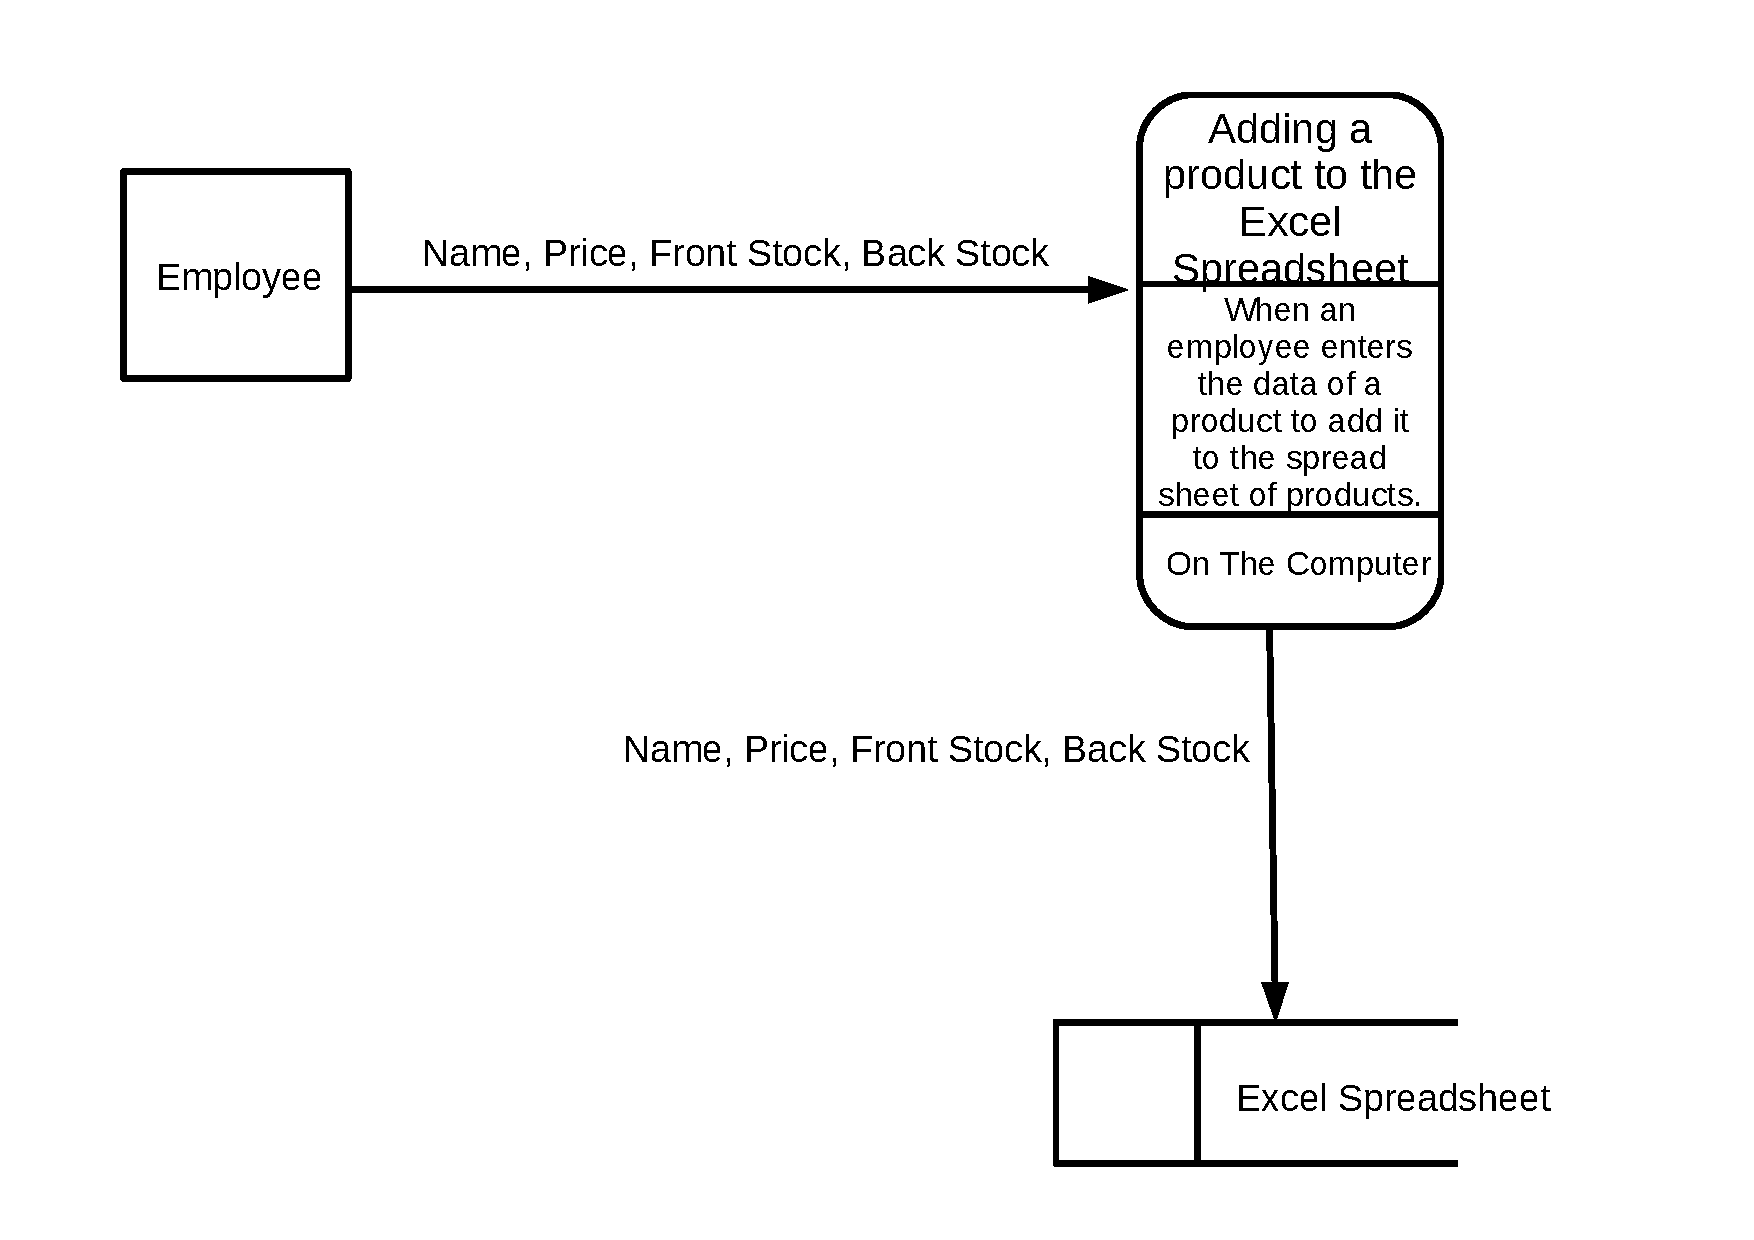
\includegraphics[width=\textwidth]{DataFlowDiagramOne.pdf}
\caption{This is the Data Flow Diagram for an employee adding a product to the database.} \label{fig:DataFlowDiagram1}
\end{figure}


\begin{figure}[H]
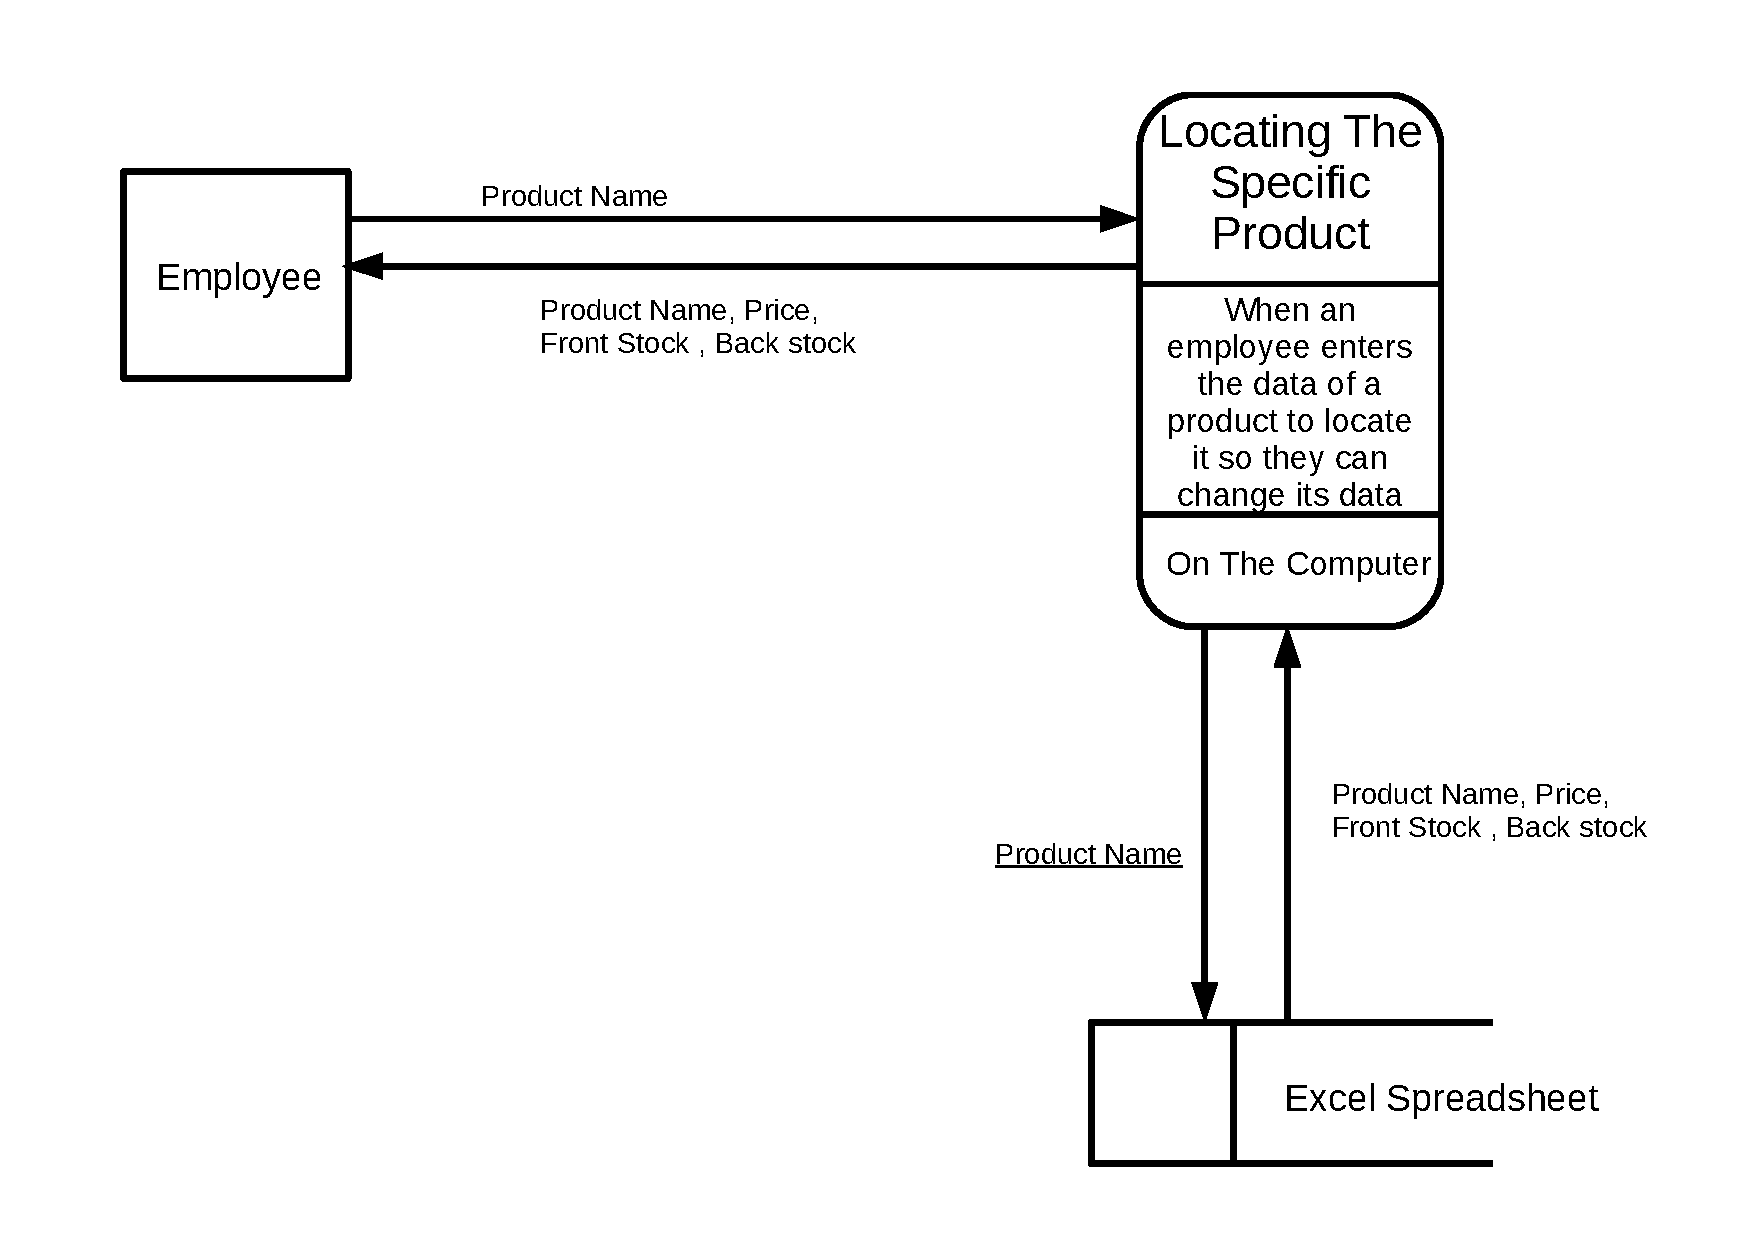
\includegraphics[width=\textwidth]{DataFlowDiagramTwo.pdf}
\caption{This is the Data Flow Diagram for a customer editing the data of an existing product..} \label{fig:DataFlowDiagram2}
\end{figure}

\subsubsection{Input Forms, Output Forms, Report Formats}

The current system only has one input form - Adding a product to the database. when a product needs to be added to the database, the product name, quantity, price and category needs to be know in order for it to be added. The product ID is automatically assigned to the item when it is added to the database. Because items are only added to the database and the information is only stored, viewed and edited when needed, there are currently no output forms for the data. In the new system, the client wants the stock control system and the selling process to be integrated. When the new system is implemented then there would be one output form which would be a receipt given to the customer when they purchase a product. The receipt would contain the following information: The Name of the product, the quantity/weight/volume of the product the quantity and the price of the product. This is so the customer knows exactly what products they bought and know how much each product costs. The Product ID is not supplied on the receipt as that information is not relevant to the customer.

\subsection{The proposed system}

\subsubsection{Data sources and destinations}

There is only one data source in the current system. Because my client wants to integrate the selling process into the current system, There will before new data sources, giving five total data sources .The first data source is when a client purchases a product or many products. The Product name, weight, quantity are entered into the new system, or a search is made into the database for the product that the customer wants to buy, when all the attributes of the product match the ones of the product stored in the database, the price of that product is taken from the database and is added to the total bill. The information entered is repeated onto a receipt that is given to the customer to clarify which items they purchased. I am not storing the data for every purchase from a customer in the new system, as there is only limited storage space and storing all the data from every purchase will require an extremely large amount of storage space. The second data source is when a new product is added to the system. This data source was used in the old system. The information about the product will be stored in the database as it is used when a customer wants to purchase a product. This information is also used when the customer wants to find a product she does not know that name of. The third data source is when the information about a product needs to be updated or edited. This new data will override the current data stored under each product and will be held inside the database. The fourth data store, is when the stock needs to changed, when an import of new stock comes in. This data will also be held inside the database.\par 
Another Data source will be when a customer supplies their MemberID if they are a member. if they are a member then they get a 10 percent discount, along with other advantages unrelated to this system. Therefore, the information about the Members of the veterinary will be stored within the database.


\subsubsection{Data flow diagram}


\begin{figure}[H]
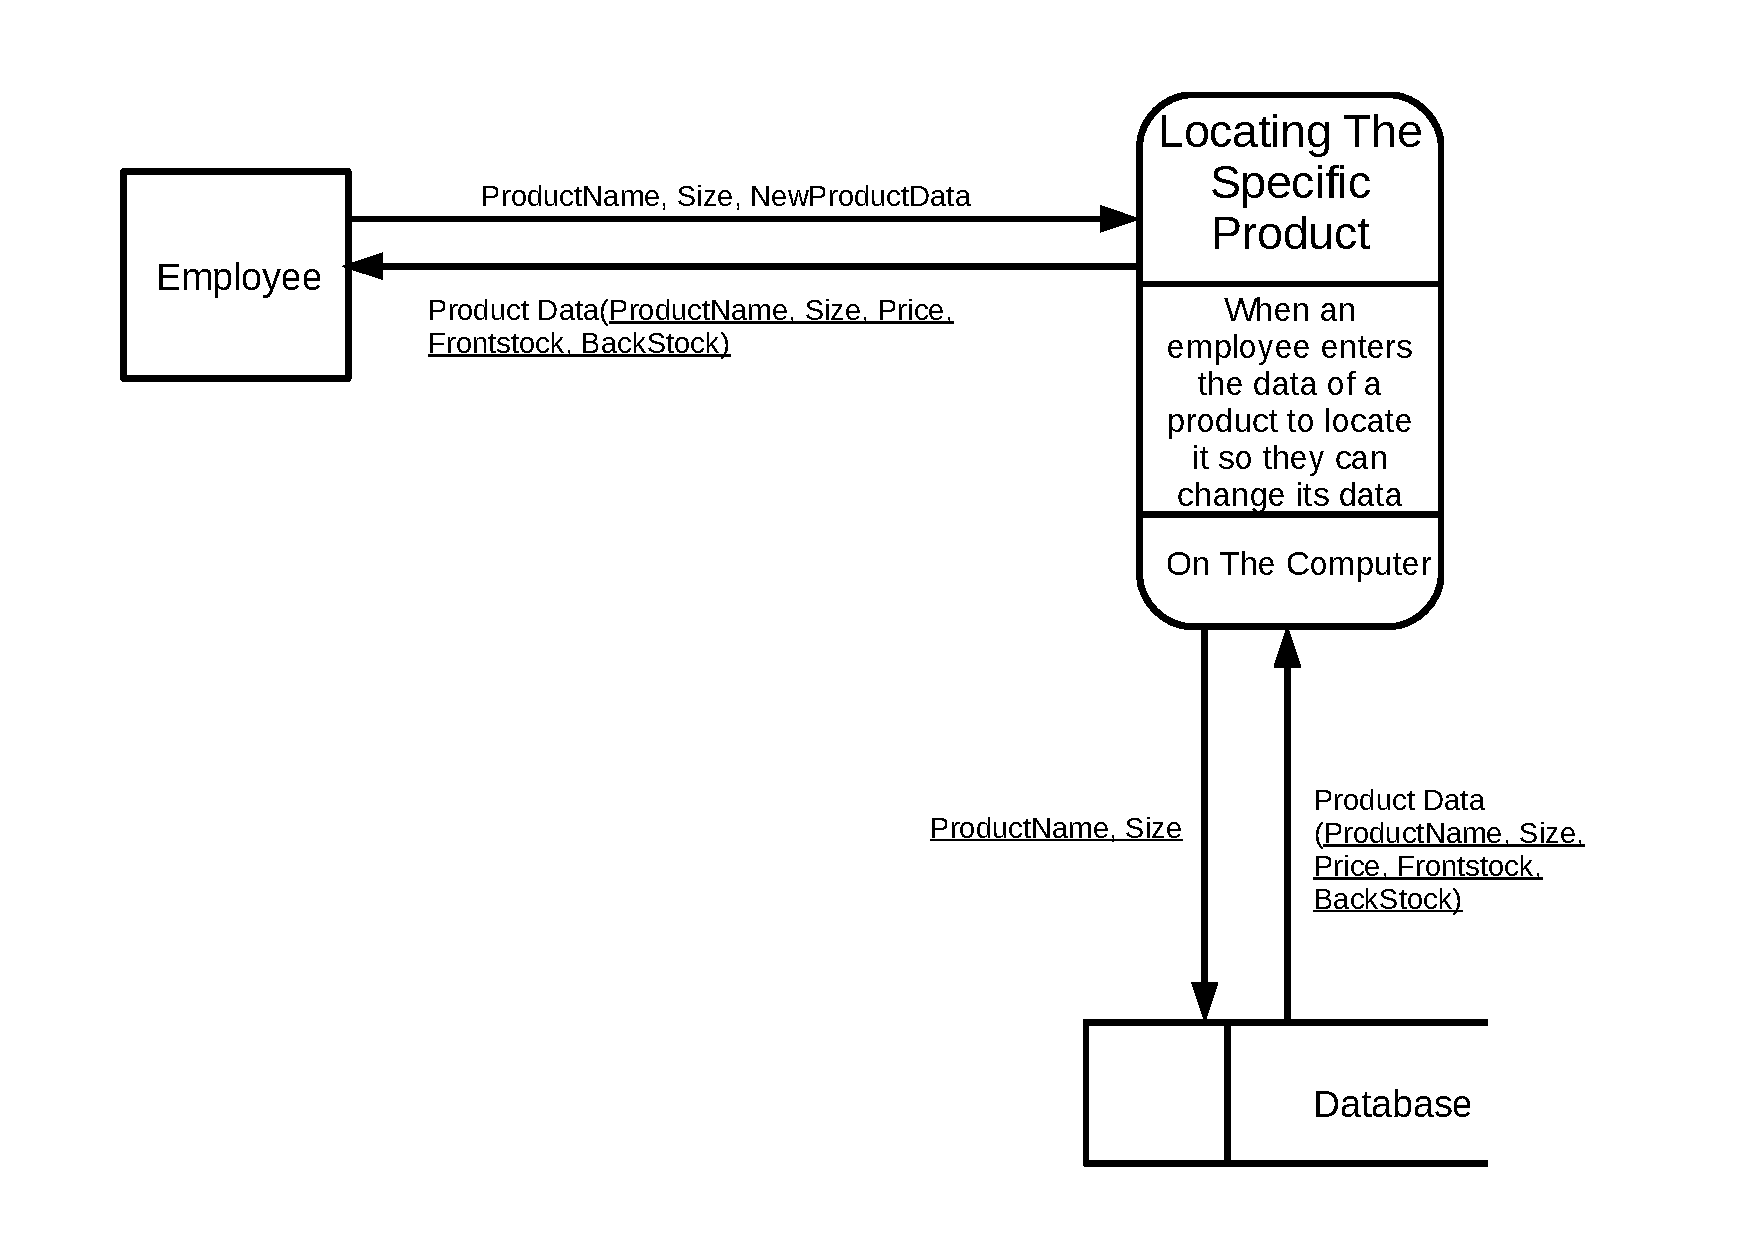
\includegraphics[width=\textwidth]{DataFlowDiagramThree.pdf}
\caption{This is the Data Flow Diagram for an employee editing the data of an existing product.} \label{fig:DataFlowDiagram3}
\end{figure}

\begin{figure}[H]
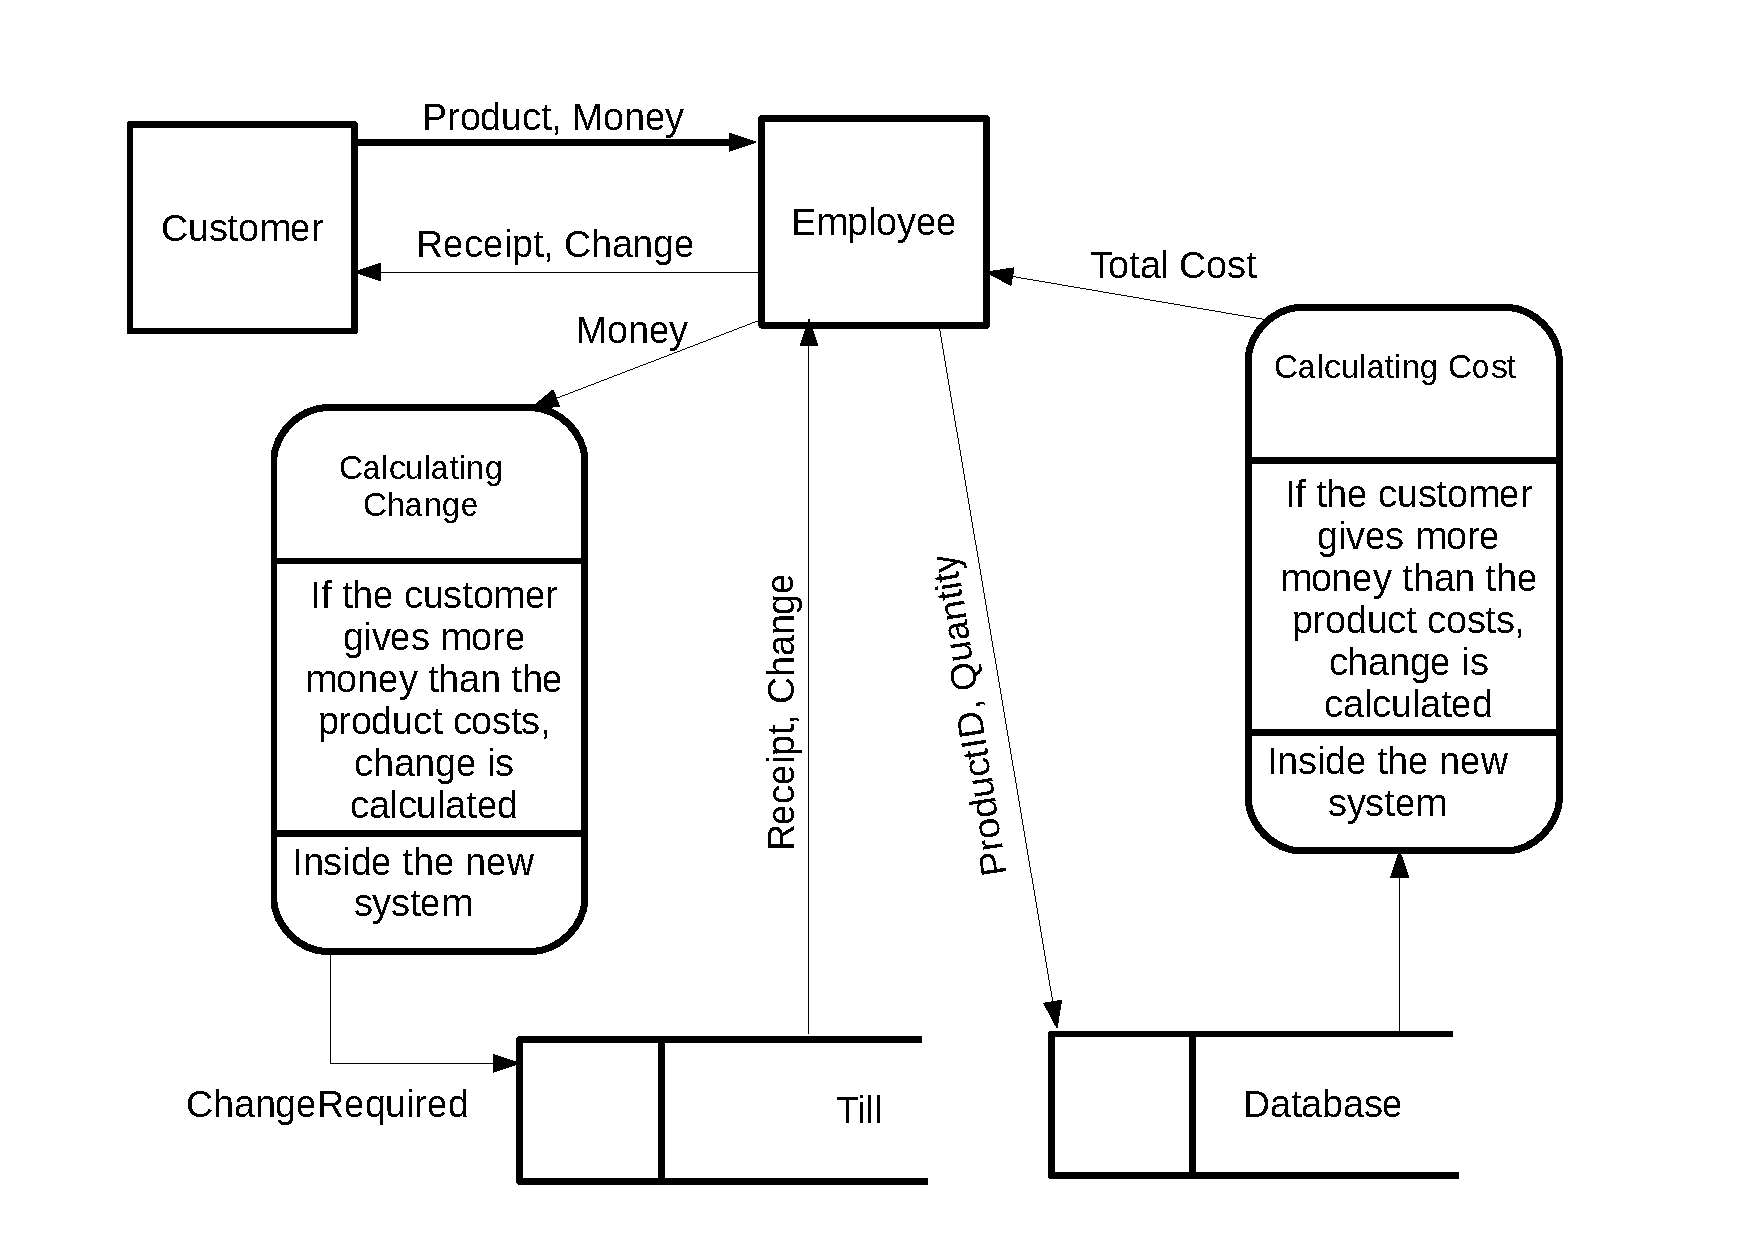
\includegraphics[width=\textwidth]{DataFlowDiagramFour.pdf}
\caption{This is the Data Flow Diagram for a customer Buying A product} \label{fig:DataFlowDiagram4}
\end{figure}

\subsubsection{Data dictionary}

\begin{center}
    \begin{tabular}{|p{3cm}|p{3cm}|p{2cm}|p{3cm}|p{3cm}|}
        \hline
        \textbf{Data} & \textbf{Data Type} & \textbf{Length} & \textbf{Validation} & \textbf{Example Data}\\ \hline
        
          ProductID & Integer & 100 & Range & 42 \\ \hline
          ProductName & String & 100 & length & OPTEX Ear Drops \\ \hline
          Size & Integer & 1000 & Range & 750 grams \\ \hline
          Price & Real & 250.00 & Range & 9.99 \\ \hline
          Catagory & String & 100 & Length & Dog food \\ \hline
          FrontStock & integer & 50 & Range & 5 \\ \hline
          BackStock & Integer & 50 & Range & 11 \\ \hline
          TotalStock & Real & 100 & Range & 20 \\ \hline
          MoneyGiven & Real & 200.00 & Range & 20.00 \\ \hline
          TotalPrice  & Real & 300.00 & Range & 20.00 \\ \hline
          ChangeRequired & Boolean & & If Money > total Price & True \\ \hline
          Change & Real & 20.00 & If Change required = True & 2.35 \\ \hline
          MemberID & Integer & 300 & Range & 24 \\ \hline
          Firstname & String & 50 & Length & Thomas \\ \hline
          LastName & String & 50 & Length & Brennan \\ \hline
          AddressFirstLine & Float & 50 & Length & 66 Market Street \\ \hline
          AddressSecondLine & Float & 50 & Length & Fordham, Ely \\ \hline
          TelephoneNumber & Integer & 11 & range & 07577209094 \\ \hline
          Email & String & 50 & Length & Example@email.com \\ \hline
          
  \end{tabular}
\end{center}

\vspace{10mm} %5mm vertical space


\begin{flushleft}
The ProductID in the new system will be created by the number that product is in the database. For example the first item to be added to the database will be assigned to ProductID = 1, the second item to be added ProductID =2 ect \ldots. Therefore, the length of the ProductID is dependent on the number of products being stored within the database. Currently, my client stores the data of 57 products. He wishes to expand to about 75 and continue to expand on this as the company grows. As a result, I have decided to set the length of ProductID to 200. This is because I want to compensate for when the company grows in size and begins to sell a lot more products. I could have decided to fix the length to 100, however I feel that this limit could be reached quite quickly.\par
The length of the ProductName has been set to 100. This seems like far too many characters needed for just a name but sometimes, some of the products have very long names.''
Aristavet Panzym Concentrated Pancreatic Enzymes Powder'' is an example of a product that has a very long name that is stored in the current database.\par
The Price has been set to a limit of 200. This seems quite high for a customer buying a few products but currently the most expensive product sold at the veterinary is''Protexin Professional Probiotics Sachets'' which is £134.95.\par
I have decided to size `size' to 1000. This seems very excessive, when it comes to quantities of products, however if the product is classified by its mass or its volume(i.e. 750g / 250ml ect \ldots) then usually the mass / volume will reach 999 grams or millilitres. Usually when it reaches 1000, it is changed into kilograms / litres.\par \textbf{1 Litre = 1000 millilitres, 1 kilogram = 1000 grams.}

\subsubsection{Volumetrics}

To calculate the \textbf{maximum} file size the system could be, i need to record the \textbf{maximum} amount of characters that arepossible to be stored within the system. (1 Byte is the amount of storage required to hold 1 character.) \par

\textit{Refer to Data Dictionary for the length of each piece of data} \par

Maximum ProductID = 3 Characters (i.e 125) = \textbf{3 Bytes}\par
Maximum ProductName = 100 Characters = \textbf{100 Bytes}\par
Maximum Size = 4 Characters (i.e 750) = \textbf{4 Bytes} \par
Maximum Price = 6 characters (assuming the `.' counts as a character') = \textbf{6 bytes} \par
Maximum Catagory  = 100 characters = \textbf{100 bytes} \par
Maximum FrontStock = 2 character (i.e 35) = \textbf{2 bytes} \par
Maximum BackStock = 2 character (i.e 21) = \textbf{2 bytes} \par
Maximum TotalStock = 3 characters (i.e 100) = \textbf{3 bytes} \par
Maximum MoneyGiven = 6 characters (assuming the `.' counts as a character') = \textbf{6 bytes} \par
Maximum TotalPrice = 6 characters (assuming the `.' counts as a character') = \textbf{6 bytes} \par
Maximum Change = 4 characters (assuming the `.' counts as a character') = \textbf{4 bytes} \par
Maximum MemberID = 3 characters = \textbf{3 bytes} \par
Maximum FirstName  = 50 characters = \textbf{50 bytes} \par
Maximum LastName  = 50 characters = \textbf{50 bytes} \par 
Maximum AdressFirstLine = 50 characters = \textbf{50 bytes} \par
Maximum AdressSecondLine = 50 characters = \textbf{50 bytes} \par
Maximum TelphoneNumber = 11 characters (assuming its a real telephone number and also assuming no intenational numbers will be stored in the database (this would require 12 characters, as the `0' at the start will have to change to +44 )) = \textbf{11 bytes} \par
Maximum Email = 50 characters = \textbf{50 Bytes} \par

Therefore, the \textbf{maximum} space required to store one Product = 3 + 100 + 4 + 6 + 100 + 2 + 2 + 3 = \textbf{220 bytes}

The maximum amount of products my client is likely to store within the new system, so the \textbf{maximum} sorage space required to store 100 products = 100 * 220 bytes = \textbf{22,000 bytes = 22Kilobytes / 22Kb}

The Amount of storage space require to hold the information concerning 1 customer = 3 + 50 + 50 + 50 + 50 + 11 + 50 = \textbf{264 bytes} \par

The maximum amount of members my client expects to have is 100. therefore The \textbf{maximum} space required to store all the memebr data = 264 * 100 = \textbf{26,400 bytes = 26.4Kilbytes / 26.4Kb} 

The Transactions made are not perminantly stored within the database, they are only temporarily used then errased. The maximum sotrage space required for a transaction = 6 + 6 + 4 = \textbf{16 bytes}


Therefore, the \textbf{maximum} storage space required (assuming the information about a transaction is currently being sotred) = 26,400 + 22,000 + 16 = \textbf{48,416 Bytes = 48.416 kilbytes / 48.416Kb}

Although it is only a very rough estimate, I used the file size of one of my previous long applications as an estimate to the file size required for the application. The file size of the application is \textbf{7,000 bytes = 7 Kilbytes / 7kb}

Finally, The \textbf{maximum} storage space, the new system could possibly need, is 48,416 + 7000 = \textbf{55416 bytes = 55.416 Kilbytes / 55.416Kb}


This amount of storage is extremely low compared to the amount of file storage available on my clients hard drive. This should mean, there should be no problem with the new system to do with not having enough memory to store the data in the database.
\end{flushleft}

\section{Objectives}

\subsection{General Objectives}

\begin{flushleft}
\begin{itemize}
\label{ref:objectives}
\item Data can be added to the database easily.
\item Data can easily be edited within the database.
\item Clear/ easy to understand the layout of the information
\item Clear/ easy to locate a product within the database
\item The system to be Clear/ easy to use.
\end{itemize}
\end{flushleft} 


\subsection{Specific Objectives}

\begin{flushleft}
\begin{itemize}
\item For an image to be displayed when an item is searched for (identifying a product if the Product information is unknown)
\item For the Stock control system to be integrated with the process of selling items. This is so that the stock is automatically updated when a product is sold.
\item For the new process of selling products to be quicker, to minimize the time for people queuing. 
\item For the current stock to automatically update when the products are bought
\item For a reminder message to pop up when stock needs to be moved from storage to the front of the vets. 
\item For each and every product to be categorised for easy identification is the Product Name and ID is unknown.
\item To calculate how much stock will be required for next month.
\item For the MemberID to be entered and the identity of the client is confirmed to make sure they are a member.
\item For Keyboard Shortcuts to be availble for the system to be acessed faster.
\item To Format a well structured receipt that is easy for the customer to read and to understand
\item allowing the Order of the products in the database to be changed.(i.e. Max - Min Price, A-Z ect \ldots)
\end{itemize}
\end{flushleft}

\subsection{Core Objectives}

\begin{flushleft}
\begin{itemize}
\item For the Stock control system to be integrated with the process of selling items. This is so that the stock is automatically updated when a product is sold.
\item For the Stock to automatically update itself.
\item To calculate how much stock will be required for next month.
\end{itemize}
\end{flushleft}

\subsection{Other Objectives}

\begin{flushleft}
\begin{itemize}
\item allowing the Order of the products in the database to be changed.(i.e. Max - Min Price, A-Z ect \ldots)
\item For Keyboard Shortcuts to be availble for the system to be acessed faster.
\item To Format a well structured receipt that is easy for the customer to read and to understand
\end{itemize}
\end{flushleft}


\section{ER Diagrams and Descriptions}

\subsection{ER Diagram}


\begin{figure}[H]
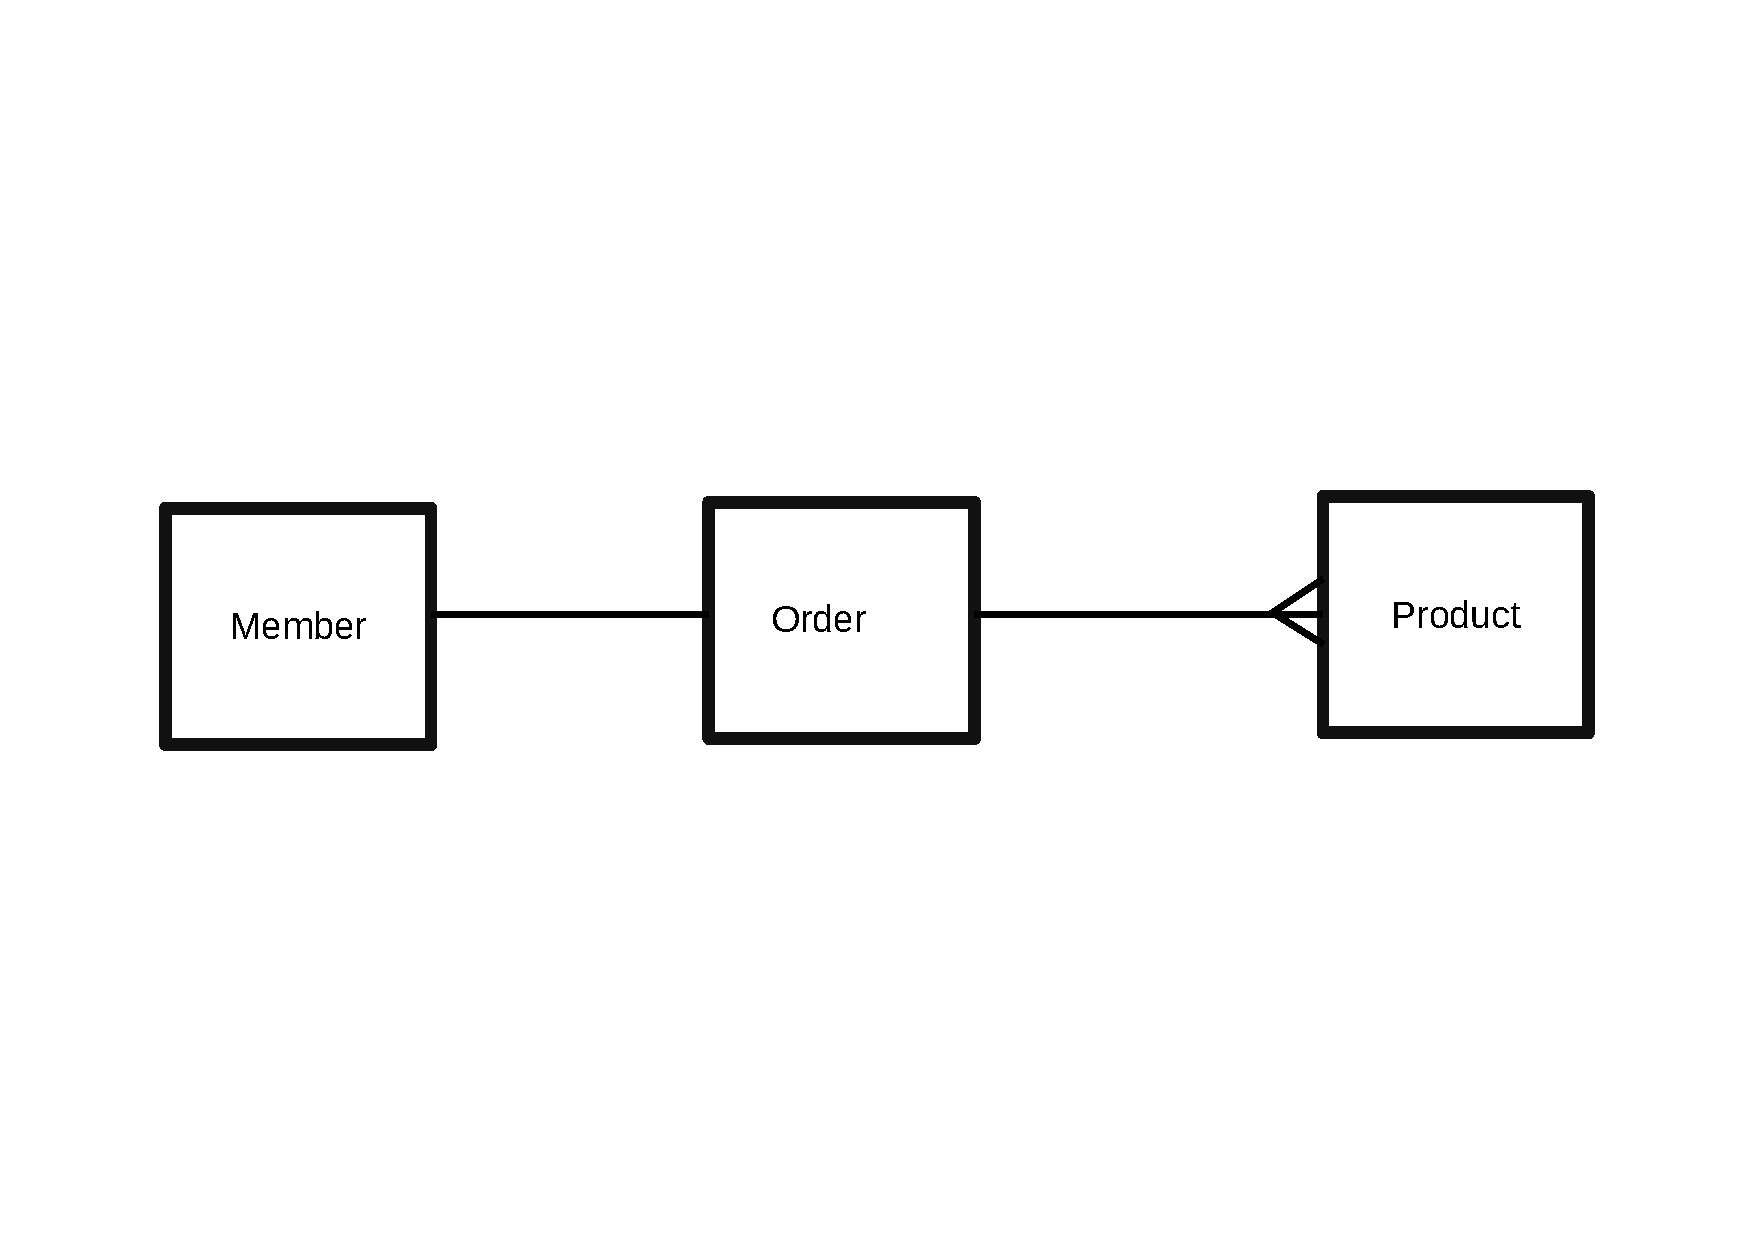
\includegraphics[width=\textwidth]{EntityRelationshipDiagram.pdf}
\caption{Entity Relationship Diagram.} \label{fig:EntityRelationshipDiagram}
\end{figure}

\subsection{Entity Descriptions}


\begin{flushleft}

Product(\underline{ProductID}, ProductName, Size, Price, Category, FrontStock, BackStock, TotalStock)

Member(\underline{MemberID}, Firstname, LastName, AddressFirstLine, AddressSecondLine, TelephoneNumber, Email.)

Order(\underline{OrderID},\textit{ProductID}, Quantity)

The relationship between order and Member is that a Member can make One Order. This order Can contain many prodcuts therefore, the relatyionship between Order and Product is one Order can have Many products. The ProductID is the primary key for Product, but is also the foreeign key for order as the ProductId is required to make an order.

\end{flushleft}

\section{Object Analysis}

\subsection{Object Listing}

\begin{flushleft}
Product(All relevant information about that product, including a unique identifier for each product.)\par
Member(All relevant information about each Member, including a unique identifier for each Member so they can identified quickly...)
Order(all relevent information about each order and the quantity of each product in that order)

\end{flushleft}
\subsection{Relationship diagrams}


\begin{figure}[H]
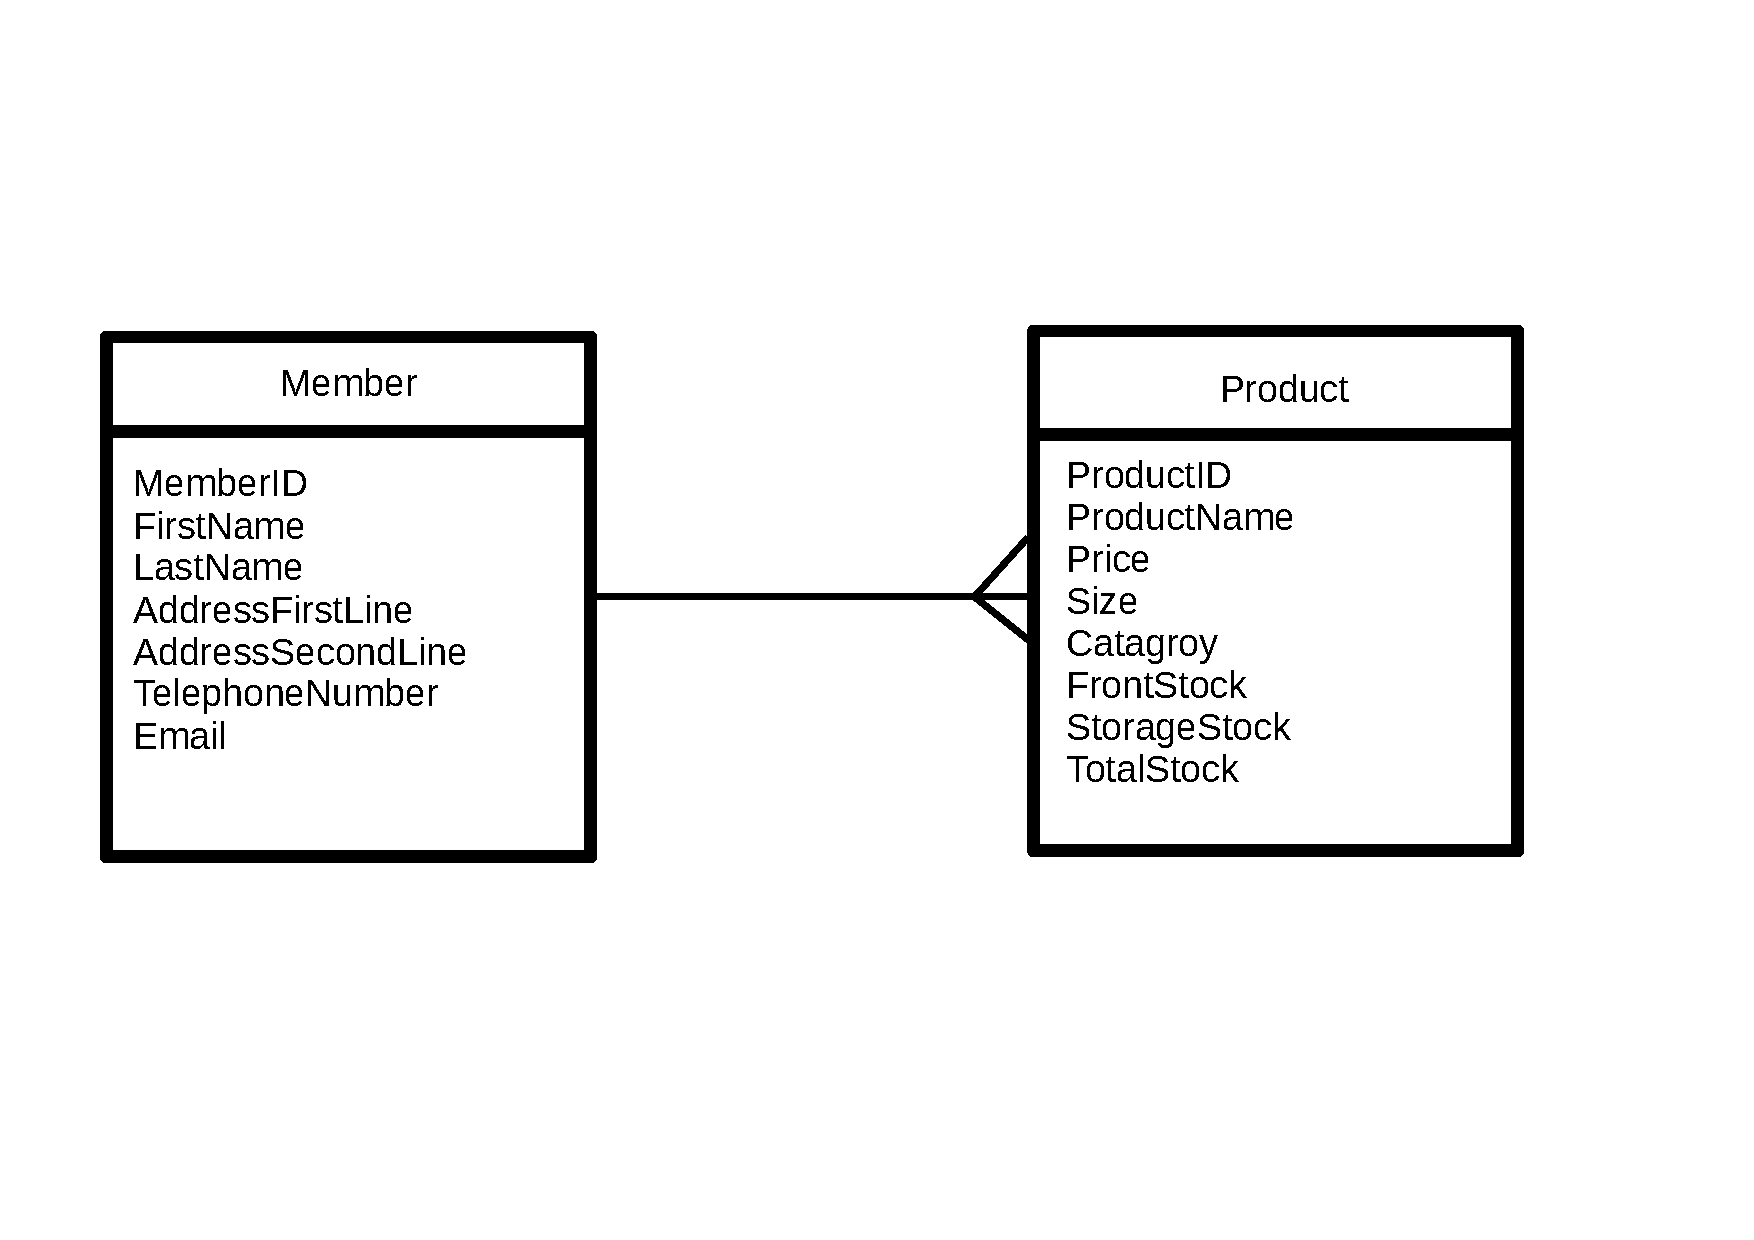
\includegraphics[width=\textwidth]{RelationshipDiagram.pdf}
\caption{A Relationship Diagram between Member and Product.} \label{fig:RelationshipDiagram}
\end{figure}

\subsection{Class definitions}

\begin{figure}[H]
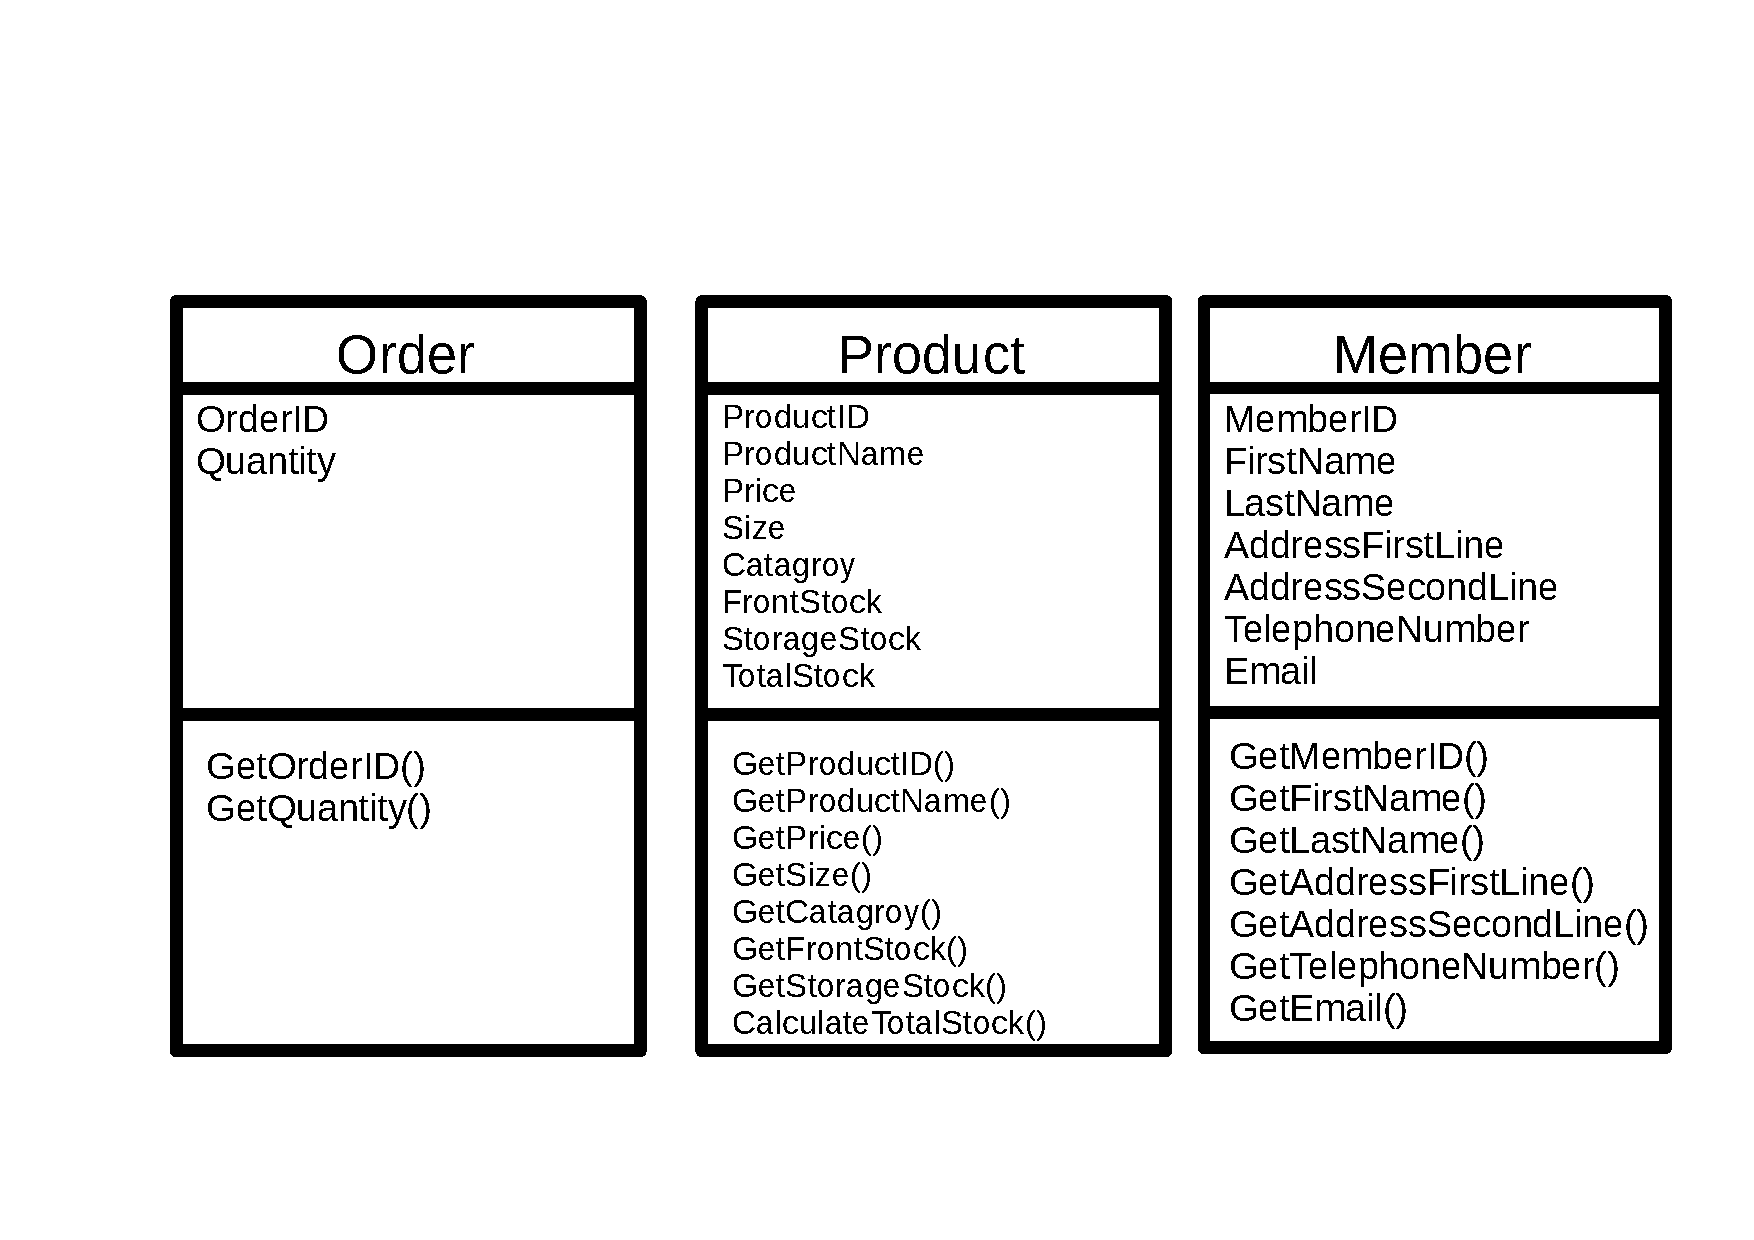
\includegraphics[width=\textwidth]{ClassDefinition.pdf}
\caption{The Class Definition For Product and Member.} \label{fig:ClassDefinition}
\end{figure}

\section{Other Abstractions and Graphs}

\begin{flushleft}
There are no current graphs to draw for the system
\end{flushleft}

\section{Constraints}

\subsection{Hardware}

\begin{flushleft}

Currently my client uses a Lenovo Desktop Pc for the current system. The computer is also used to check emails and to check appointment times with customers. The new system will be able to run on this machine.

Computer Specifications:

\begin{itemize}
\item{21'' LCD Monitor}
\item{Intel® Core™ i3-3240T processor}
\item{4 GB DDR3}
\item{1 TB HDD, 7200 rpm}
\item{H61 Motherboard}
\end{itemize}

The demand of the purposed system will make little to no impact on the Computers speed. The requirements for the purposed system is far less than the current hardware can provide meaning there will be no problem running the new system on this computer. \par

Although the proposed system will be able to run on this computer there are a few hardware constraints. One of which is that the fact this computer is a desktop computer. This means that my client will not be able to move this system and will have to keep the computer in one place. This is because the desktop computer does not have an internally stored battery. \par

Another Hardware constraint is that the new system will have to be designed and implemented to fit the screen resolution of my clients computer. \par

\end{flushleft}


\subsection{Software}

\begin{flushleft}
My client currently uses Microsoft Excel as his system. Tom is happy to use any other software. Because Tom takes full ownership of the computer he has no limitations on what he would like to install. for example if the computer belonged to someone else, the user of the computer would want as little changes as possible. Tom's computer currently runs Windows 7 Home Edition, which the new system will be able to run on. The only software constraint is that if my client were to buy a new computer with a different operating system, the new system may not be cross compatible with the new operating system. This would mean the new system will have to be completely recreated to work on the new operating system. Another Software constrait which is unlikely but possible, is that updating the operating system to a newer version may cause problems with the new system.
\end{flushleft}

\subsection{Time}

\begin{flushleft}
My client has set no deadline or time limit for the completion of the system. The only time restriction I have on this project is the deadline set by my teacher, which is the end of February. Tom says he is happy to start using the new system when it is ready. The sooner it is finished the better.
\end{flushleft}

\subsection{User Knowledge}

\begin{flushleft}
At this current time tom does not have any qualifications in ICT and has not taken any IT courses. Despite this, Tom has a quite good knowledge when it comes computers, Gaining most of his knowledge whilst doing his Veterinary Medicine degree. He has helped devolve web pages, and is currently helping create a new website for Beacon Vets. However Tom informed me that he would not be the only one to be using the system, It will also be used by the receptionists when customers buy products. This means that The interface has to easy for easy for begginers or people who have less of an understand of computers than Tom to use. 
\end{flushleft}

\subsection{Access restrictions}

\begin{flushleft}
There proposed system should be accessible to anyone that works at beacon vets. Every employee will have full access/privileges to all of the data on the system. The computer will be password protected along with the system to prevent unwanted users on the computer to access the database, and potentially erase or edit all of the data within the database. \par
Because the database stores personal information about people, the system has to follow to Data Protection Act. Tom and all the employees at Beacon Vets will have to be informed of this law in hope they do not break it.However the system can be designed to follow to Data Protection Act, meaning that Tom and the emplyees do not have to warry about breakign this Law.
\end{flushleft}

\section{Limitations}

\subsection{Areas which will not be included in computerisation}

\begin{flushleft}
Areas that shall not be included in computerisation is the exchange of money when products are brought. Currently, The vets allows two method of payment. The two methods of payment are by cash or by Credit / Debit card. The proposed system will only handle information from customers that pay by cash.(i.e. Calculating change ect \ldots) The proposed system will not handle data from customers who pay by card because that information is handled externally by an external card reader, which will be too complicated to integrate into my new system. \par 

The process of moving products form storage to the front of the vets obviously will not be computerised. This will be done externally, and a tick box will be supplied by the system for the employee to tick when the products have been moved. The limitation with this is that the system will assume the employee has moved the correct amount of products. \par

When adding a new product to the system the data will be input manually. Although this is not part of the system, teaching Tom how to use the new system will not be computerised. Tom would then have to use the knowledge I have taught him and teach all of the employees at Beacon Vets.
\end{flushleft}

\subsection{Areas considered for future computerisation}

\begin{flushleft}
An area that could be computerised is teaching tom / the employees, on how to use the new system. Written instructions could be processed into a document for a employee to refer to if they need to do something, but do not currently know how. This will mean that Tom will not have to take time out explaining how to use the system to each and every employee. He can send an email with the instructions attached to it for each of the employees to read and the instructions document could be easily accessible in the system if they forget / don't know how to do something. The process of moving products using a computer is not possible. The process of selling product can be computerised by creating a page on the website where customers can buy the products online. This could be possible as the location of Beacon Vets (Silloth) is a small town and is mainly only used by the local community. This is useful because it means that product deliveries can be made within a maximum of 10 miles from the store. The limitations with computerising this method is that creating a web page like this is that I do not currently have the skill sets to create a webpage like this. The webpage will have to be secure, and will have to have things such as PayPal incorporated into it. To prevent the customers from having to enter their card details in every time they make a purchase, their card details will have to be stored on the system. This will then mean that the system will have to abide by the data protection act, however I feel this information can be stored securely over PayPal, which will reduce the problems faced when creating the system.
\end{flushleft}

\section{Solutions}

\subsection{Alternative solutions}



\begin{center}
\begin{tabular}{|p{4cm}|p{4cm}|p{4cm}|}
\hline
\textbf{Solution} & \textbf{Advantages} & \textbf{Disadvantages} \\ \hline
{Custom Spread Sheet} & {My client already uses a spreadsheet software called "Microsoft Excel",
so no training is required.\par No new software will have to be downloaded.} & {my client uses spreadsheet software for his current system. He explains that the system is easy and simple to mange with a few products but as time went by and more products were added it because difficult, unordered and confusing.} \\ \hline
{Web Based Application} & {the information stored in the database can be stored in the cloud. This would reduce the file size of the system.\par The system can be accessed on more than one computer and no information has to be installed.} & {Data is not as secure if it is stored in the cloud. It is possible for someone to intrude into your database and modify the data. This would be less likely if the data was stored on a hard drive as the information could only be accessed on that one computer in which the hard drive is in.\par The system would have to constantly be online, meaning that there would have to be more security measures to prevent data theft.\par Hosting the web application will be more expensive than having a program. A lot more knowledge in building the web based system compared to using a program.\par} \\ \hline
{Re-organising/ re designing the current manual system} & {Would take a small amount of time to create.\par No New software will need to be installed.\par No new skills will have to be taught to the employees.\par } & {The problem my client currently has may not be overcome.\par Very simple system that is hard to change.} \\ \hline
{Command-line Application} & {Easier to design and program compared to a gui application.\par often runs faster than any gui application.\par I believe less computer resources would be used compared to using a GUI application} & {Command line applications are not user friendly when sued by people with little computer knowledge.\par Many of the employees will have had little / no training using command line applications.\par A lot of error checking will have to be implemented so that the user does not accidently crash the application.\par commands used in using the command line application takes time to remember and takes time to learn how to use the application.} \\ \hline
{Python Desktop Application with a GUI} & {The application can be designed so that extremely little amounts of training are needed to use the application.\par the client can design their own layout or design.\par The data can be displayed in a organised and visually attractive way.\par The data in the application can be easily formatted / edited.} & {It takes longer to create a gui application compared to a command line application.\par a lot of time needs to be spent on finding a good layout for the system. Using a Python desktop application with a GUI will require more computer resources compared to a command line application.} \\ \hline
\end{tabular}
\label{tab:range_examples}
\end{center}

\subsection{Justification of chosen solution}

\begin{flushleft}
I have chosen to use a "Python Desktop Application including a GUI" for my system, this is because:\par
\end{flushleft}

\begin{enumerate}
\item I Already know the Python programming language, which will reduce time in me having to learn how to create the system.
\item I know a very limited amount of HTML and don't have any knowledge on any other web based languages, so I would have to take a lot of time out to learn about how to use HTML to create the Web based application and how to integrate it with things such as PayPal and The Cloud ect \ldots
\item I can use a tool called 'Git' to back up my work so if I do have a problem, I can just roll back to my last saved piece of work. Git also allows me to see the changes I have made since I last updated my system so I can see where the errors have been created if they occur.
\item The new system will be simple and easy to use which will mean my client and his employees will not have to spend much time learning how to use the new system.
\item Using a Python application with a GUI is a lot easier to use compared to a command line application where my client and his employees will have to learn commands to use in the system.
\end{enumerate}
